\documentclass[oneside,11pt,parskip=half,ngerman]{scrreprt}
%\documentclass[a4paper,oneside,11pt,parskip=half,ngerman]{scrreprt}
\usepackage{typearea}

\usepackage[ngerman]{babel}
\usepackage[colorlinks=false, pdfborder={0 0 0}]{hyperref}
\usepackage{multirow}
\usepackage{booktabs}
\usepackage[utf8]{inputenc}
\usepackage[T1]{fontenc}
\usepackage{charter}
\usepackage[expert]{mathdesign}

\usepackage{listings}
\usepackage{xcolor}
\usepackage{color}
\usepackage{fancyhdr}
\usepackage{rotating}
\usepackage{titlesec}
\usepackage{mathptmx}
\usepackage{amssymb} % checkmark
% \usepackage{helvet}
\usepackage[scaled]{uarial}
\renewcommand*\familydefault{\sfdefault} %% Only if the base font of the document is to be sans serif
\usepackage[squaren]{SIunits}
\usepackage{graphicx}
\usepackage{url}
\usepackage{geometry}
\usepackage[absolute]{textpos}
\usepackage{makeidx}
\usepackage{colortbl}
\usepackage{pdflscape}
\usepackage{pdfpages}
\usepackage{tabularx}
\usepackage{lmodern}
\usepackage{longtable}
\usepackage{array}
\usepackage{float}
\usepackage{scrhack}
\usepackage{fancyhdr}
\usepackage{fancyvrb}

\usepackage[section]{placeins}

\usepackage{pdfpages}

\usepackage[firstpage]{draftwatermark}

%Typesetting
\usepackage[activate=true,final,tracking=true,kerning=true,spacing=true,factor=1100,stretch=10,shrink=10]{microtype}
\SetProtrusion{encoding={*},family={bch},series={*},size={6,7}}
              {1={ ,750},2={ ,500},3={ ,500},4={ ,500},5={ ,500},
               6={ ,500},7={ ,600},8={ ,500},9={ ,500},0={ ,500}}

% Bibliography
\usepackage[backend=bibtex]{biblatex}
\usepackage{csquotes}
\bibliography{./Citer}


%define page margin
\geometry{a4paper, top=30mm, left=30mm, right=30mm, bottom=30mm,headsep=10mm,footskip=10mm}

\usepackage{tocloft}
\setlength\cftbeforetoctitleskip{-2.5em}
\setlength\cftbeforeloftitleskip{-2.5em}
\setlength\cftbeforelottitleskip{-2.5em}




\usepackage{graphicx}
% We will generate all images so they have a width \maxwidth. This means
% that they will get their normal width if they fit onto the page, but
% are scaled down if they would overflow the margins.
\makeatletter
\def\maxwidth{\ifdim\Gin@nat@width>\linewidth\linewidth
\else\Gin@nat@width\fi}
\makeatother
\let\Oldincludegraphics\includegraphics
\renewcommand{\includegraphics}[1]{\Oldincludegraphics[width=\maxwidth,height=20em,keepaspectratio]{#1}}


% Chapter styling
\usepackage[grey]{quotchap}
\makeatletter 
\renewcommand*{\chapnumfont}{%
  \usefont{T1}{\@defaultcnfont}{b}{n}\fontsize{80}{100}\selectfont% Default: 100/130
  \color{chaptergrey}%
}
\makeatother

\begin{titlepage}
\title{\bigskip \bigskip Evaluation von Synchronisations- und Konfliktlösungsverfahren im
Web-Umfeld}
\author{Martin Eigenmann}

%\include{../content/Titelblatt.tex}
%
\includepdf[pages=1]{../content/Titelblatt}

\end{titlepage}

\begin{document}  
\maketitle

\pagenumbering{roman}

\chapter{Abstract}\label{abstract}

\chapter{Danksagungen}\label{danksagungen}

Thanks Mum.\\Thanks Dad.\\\ldots{}

\setcounter{tocdepth}{1}

\chapter{Inhaltsverzeichnis}\label{inhaltsverzeichnis}

\renewcommand{\contentsname}{} 

\begingroup\let\clearpage\relax
\tableofcontents
\endgroup

\microtypesetup{protrusion=true}

\newpage

\pagenumbering{arabic}

\part[Teil i]{Einleitung und Abgrenzung}

\chapter{Einleitung}\label{einleitung}

\section{Motivation und
Fragestellung}\label{motivation-und-fragestellung}

Der Zugriff auf Services und Medien mittels mobiler Geräte steigt
beständig an. So ist im Mai 2014, 60\% der Zeit, die online verbracht
wird, über Handy und Tablet zugegriffen worden - davon 51\% mittels
mobiler Applikationen. \autocite{comescore-mobiletrends}

\begin{figure}[htbp]
\centering
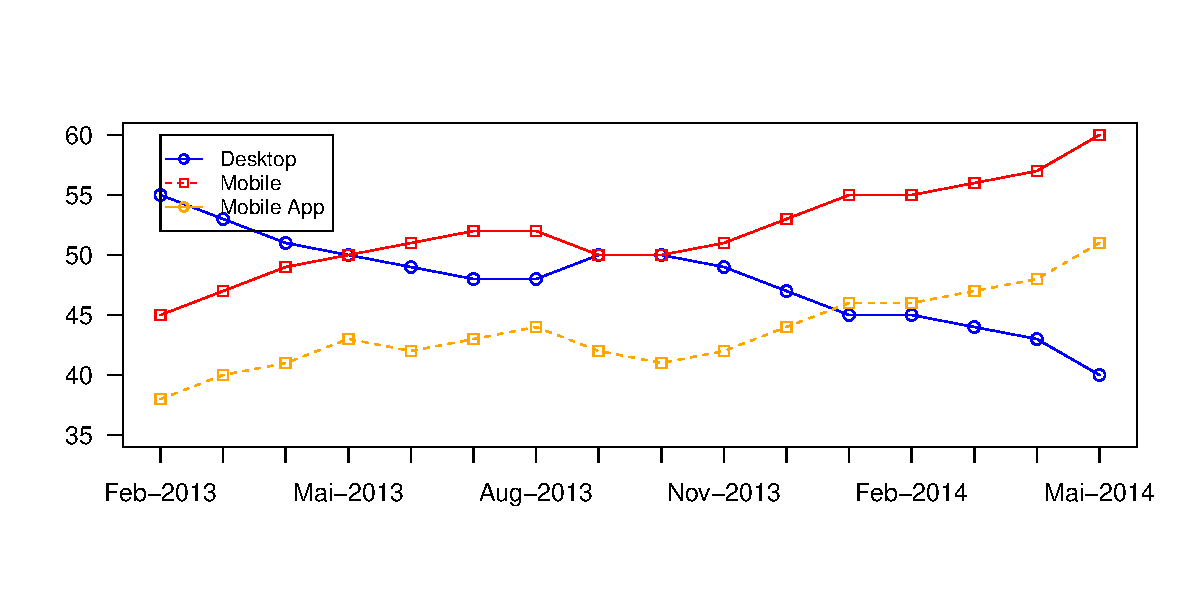
\includegraphics{img/Share-of-US-Digital-Media-Time-Spent-by-Platform.pdf}
\caption{Verteilung der online verbrachten Zeit nach Platform (Grafik
erstellt gemäss der Daten von \autocite{comescore-mobiletrends})}
\end{figure}

Angesichts der grossen Verbreitung und Nutzung von Services und Medien
im Internet, wird eine unterbruchsfreie Benutzbarkeit, auch ohne
Internetverbindung, immer selbstverständlicher und somit auch immer
wichtiger.

\begin{quote}
\enquote{It's clear that the mobile industry has finally given up on the
fantasy that an Internet connection is available to all users at all
times. Reality has set in. And in the past month, we've seen a new wave
of products and services that help us go offline and still function.}
\textcite{cw-mobiletrends}
\end{quote}

Es stellt sich nun die Frage, wie Informationen, über
Verbindungsunterbrüche hinweg, integer gehalten werden können. Und wie
Daten im mobilen Umfeld synchronisiert, aktualisiert und verwaltet
werden könne, so dass für den Endbenutzer schlussendlich kein
Unterschied zwischen Online- und Offline-Betrieb mehr wahrnehmbar ist.

\section{Aufgabenstellung}\label{aufgabenstellung}

Die von der Leitung des Studiengangs Informatik freigegebene
Aufgabenstellung ist im Appendix unter
\enquote{\hyperref[appendixux5faufgabenstellung]{Aufgabenstellung}}
aufgeführt.

\section{Abgrenzung der Arbeit}\label{abgrenzung-der-arbeit}

\section{Begründung}\label{begruxfcndung}

\section{Geschichtliche Einordnung in das
Thema}\label{geschichtliche-einordnung-in-das-thema}

\chapter{Dokumentationsstruktur und Beitrag zum
Forschungsgebiet}\label{dokumentationsstruktur-und-beitrag-zum-forschungsgebiet}

\emph{Teil i - Einleitung und Abgrenzung}

\emph{Teil ii - Technische Grundlagen und Architekturen}

\emph{Teil iii - Konzept und Implementierung}

\emph{Teil iv - Abschluss und Ausblick}

\part[Teil ii]{Technische Grundlagen und Architekturen}

\chapter{Recherche}\label{recherche}

Dieses Kapitel erklärt die wichtigsten Grundbegriffe und wiedergibt die
während der Recherche gesammelten Informationen.

\section{Fachbegriffe}\label{fachbegriffe}

Eine Aufführung und Erlährung der Fachbegriffe befindet sinch im
Appendix unter \enquote{\hyperref[glossar]{Glossar}}

\section{Erläuterung der
Grundlagen}\label{erluxe4uterung-der-grundlagen}

\subsection{Datenbanken}\label{datenbanken}

Eine Datenbank \footnote{In der Literatur oft auch als
  \textbf{D}aten\textbf{B}ank\textbf{S}ystemen (DBS) oder
  Informationssystem bezeichnet. \autocite[ pp.~3-4]{rupDatenbanken}}
ist ein System zur Verwaltung und Speicherung von strukturierten Daten.
Erst durch den Kontext des Datenbankschemas wird aus den Daten
Informationen, die zur weiteren Verarbeitung genutzt werden können. Ein
Datenbanksystem umfasst die beiden Komponenten Datenbankmanagementsystem
(DBMS) sowie die zu veraltenden Daten selbst.\\Ein DBMS muss die vier
Aufgaben \footnote{Bekannt als ACID-Prinzip \autocite[
  pp.105]{rupDatenbanken} umfasst es \textbf{A}tomicity,
  \textbf{C}onsistency, \textbf{I}solation und \textbf{D}urability.}
erfüllen.

\begin{itemize}
\itemsep1pt\parskip0pt\parsep0pt
\item
  Atomarität
\item
  Konsistenzerhaltung
\item
  Isolation
\item
  Dauerhaftigkeit
\end{itemize}

Neben den vielen neu auf den Markt erschienen Technologien wie Document
Store oder Key-Value Store ist das Relationale Datenbankmodell immer
noch am weit verbreitet. \autocite{dbenginesranking}.

\subsection{Monolithische Systeme}\label{monolithische-systeme}

Als Monolithisch wird ein logisches System bezeichnet, wenn es in sich
geschlossen, ohne Abhängigkeiten zu anderen Systemen operiert. Alle zur
Erfüllung der Aufgaben benötigten Ressourcen sind im System selbst
enthalten. Es müssen also keine Ressourcen anderer Systeme alloziert
werden und somit ist auch keine Kommunikation oder Vernetzung
notwendig.\\Das System selbst muss jedoch nicht notwendigerweise aus nur
einem Rechenknoten bestehen, sondern darf auch als Cluster implementiert
sein.

\subsection{Verteilte Systeme}\label{verteilte-systeme}

Man kann zwischen physisch und logisch verteilten Systemen
unterscheiden. Weiter kann das System auf verschiedenen
Abstraktionsstufen betrachtet werden. So sind je nach Betrachtungsvektor
unterschiedliche Aspekte relevant und interessant.
\autocite{ethdistribsystems}

\subsubsection{physisch verteilte
Systeme}\label{physisch-verteilte-systeme}

Rechnernetze und Cluster-Systeme werden typischerweise als physisch
verteiltes System betrachtet. Die Kommunikation zwischen den einzelnen
Rechenknoten erfolgt nachrichtenorientiert und ist somit asynchron
ausgelegt. Jeder Rechenknoten verfügt über exklusive Speicherressourcen
und einen eigenen Zeitgeber.\\Durch die Implementation eines Systems
über mehrere unabhängige physische Rechenknoten kann eine erhöhte
Ausfallsicherheit und/oder ein Performance-Gewinn erreicht werden.

\subsubsection{logisch verteilte
Systeme}\label{logisch-verteilte-systeme}

Falls innerhalb eines Rechenknoten echte Nebenläufigkeit\footnote{Von
  echter Nebenläufigkeit wird gesprochen, wenn verschiedene Prozesse zur
  selben Zeit ausgeführt werden. (Multiprozessor)} oder
Modularität\footnote{Modularität beschreibt die Unabhängigkeit und
  Austauschbarkeit einzelner (Software-) Komponenten. (Auch Lose
  Kopplung gennant)} erreicht wird, kann von einem logisch verteilten
System gesprochen werden. Einzelne Rechenschritte und Aufgaben werden
unabhängig voneinander auf der selben Hardware ausgeführt. Dies
ermöglicht den flexiblen Austauschen\footnote{Austauschbarkeit einzelner
  Programmteile wird durch die Einhaltung der Grundsätze von modularer
  Programmierung erreicht.} einzelner Aufgaben.

\subsection{Verteilte Algorithmen}\label{verteilte-algorithmen}

Verteilte Algorithmen sind Prozesse welche miteinander über Nachrichten
(synchron oder asynchron) kommunizieren und so idealerweise ohne
Zentrale Kontrolle eine Kooperation erreichen.
\autocite{ethdistribalgo}\\Performance-Gewinn, bessere Skalierbarkeit
und eine breitere Abdeckung der unterstützen von verschiedenen
Hardware-Architekturen kann durch den Einsatz von verteilten Algorithmen
erreicht werden.

\subsection{Verteilte Datenbanken}\label{verteilte-datenbanken}

{[}Präsenzbibliothek ZHAW{]}

\subsection{Replikation}\label{replikation}

Replikation vervielfacht ein sich möglicherweise mutierendes Objekt
(Datei, Dateisystem, Datenbank usw.), um hohe Verfügbarkeit, hohe
Performance, hohe Integrität oder eine beliebige Kombination davon zu
erreichen. \autocite[ p.~19]{SWB-327013990}

\hyperdef{}{synchrone-replikation}{\subsubsection{Synchrone
Replikation}\label{synchrone-replikation}}

Eine synchrone Replikation stellt sicher, dass zu jeder Zeit der gesamte
Objektbestand auf allen Replikationsteilnehmern identisch ist.

Wird ein Objekt eines Replikationsteilnehmer mutiert, wird zum
erfolgreichen Abschluss dieser Transaktion, von allen anderen
Replikationsteilnehmern verlangt, dass sie diese Operation ebenfalls
erfolgreich abschliessen.\\Üblicherweise wird dies über ein
Primary-Backup Verfahren realisiert. Andere Verfahren wie der
2-Phase-Commit und 3-Phase-Commit ermöglichen darüber hinaus auch das
synchrone Editieren von Objekten auf allen Replikationsteilnehmern.
\autocite[ p.~23ff, 134ff]{SWB-327013990}

\subsubsection{Asynchrone Replikation}\label{asynchrone-replikation}

Eine asynchrone Replikation, stellt periodisch sicher, dass der gesamte
Objektbestand auf allen Replikationsteilnehmern identisch ist.
Mutationen können nur auf dem Master-Knoten durchgeführt werden. Einer
oder mehrere Backup-Knoten übernehmen dann periodisch die
Mutationen.\\Entgegen der \hyperref[synchrone-replikation]{synchronen
Replikation} müssen nicht alle Replikationsteilnehmer zu jedem Zeitpunkt
verfügbar sein\footnote{So kann der Backup-Knoten nur Nachts über
  verfügbar sein, damit die dazwischen liegende Verbindung Tags über
  nicht belastet wird.}.

\subsubsection{Merge Replikation}\label{merge-replikation}

Die merge Replikation erlaubt das mutieren des Objekts auf einem
beliebigen Replikationsteilnehmer.\\Mutationen auf einem einzelnen
Replikationsteilnehmer werden periodisch allen übrigen
Replikationsteilnehmern mitgeteilt. Da ein Objekt
zwischenzeitlich\footnote{Zwischen der lokalen Mutation und der
  Publikation dieser an die übrigen Replikationsteilnehmer, liegt eine
  beliebige Latenz.} auch auf anderen Teilnehmern mutiert worden sein
kann, müssen während des Synchronisationsvorgang\footnote{Da die
  Replikation nicht notwendigerweise nur unidirektional, sondern im
  Falle von einem Multi-Master Setup auch bidirektional durchgeführt
  werden kann, wird hier von einer Synchronisation gesprochen.}
eventuell auftretenden Konflikte aufgelöst werden.

\subsection{Block-Chain}\label{block-chain}

Die Block-Chain ist eine verteilte Datenbank die ohne Zentrale Kontrolle
auskommt. Jede Transaktion wird kryptographisch gesichert, der Kette von
Transaktionen hinzugefügt. So ist das entfernen oder ändern
vorhergehender Einträge nicht mehr möglich\footnote{Das ändern
  vorhergehender Einträge benötigt mehr Rechenzeit, als alle anderen
  Teilnehmer ab diesem Zeitpunkt zusammen aufgewendet haben.}. Jeder
Teilnehmer darf also alle Einträge lesen und neue Einträge hinzufügen.
Da Einträge nur hinzugefügt werden und nie ein Eintrag geändert wird,
kann eine Block-Chain immer ohne Synchronisationskonflikte repliziert
werden. Konflikte können nur in den darüberlegenden logischen
Schichten\footnote{So prüft die Bitcoin-Implementation ob eine
  Transaktion (Überweisung eines Betrags) bereits schon einmal
  ausgeführt wurde, und verweigert gegebenenfalls eine erneute
  Ausführung.} auftreten. \autocite{block-chain}

\hyperdef{}{analyse}{\chapter{Analyse}\label{analyse}}

\section{Datenanalyse}\label{datenanalyse}

Daten können bezüglich ihrer Beschaffenheit, Geltungsbereich und
Gültigkeitsdauer unterschieden werden. Dabei spricht man von der
Klassifikation. Es werden nur die in den Daten enthaltenen Informationen
dafür herangezogen. Die Form der Daten, also der Datentyp selbst ist für
die Klassifikation unerheblich.

Die Datentypisierung unterscheidet zwischen numerischen (num), binären
(bin), logischen (bool) und textuellen (text) Daten.

Eine Attributsgruppe, also eine logische Aufteilung der Informationen in
mehrere Attribute ist eine zusammenhängende Informationseinheit.

\subsection{Kontextbezogene Daten
(Struktur)}\label{kontextbezogene-daten-struktur}

Daten die nur in einem bestimmten Kontext einen signifikanten
Informationsgehalt aufweisen, der ohne Kontext nicht greifbar ist,
werden als kontextbezogene Daten bezeichnet.\\(Kommentar auf einen
Artikel)\\

\subsection{Unabhängige Daten
(Struktur)}\label{unabhuxe4ngige-daten-struktur}

Mit dem Begriff der unabhängigen Daten werden all jene Datensätze
bezeichnet die in sich abgeschlossene Informationen
beinhalten.\\(Artikel)

\subsection{Exklusive Daten (Art)}\label{exklusive-daten-art}

Exklusive Daten sind Daten und Datensätze die nur von einem Aktor
bearbeitet werden dürfen.\\(Wecker-Einstellungen)

\subsection{Gemeinsame Daten (Art)}\label{gemeinsame-daten-art}

Daten die von mehreren Aktoren gleichzeitig gelesen und bearbeitet
werden dürfen, werden als gemeinsame Daten
bezeichnet.\\(Firmen-Todo-Liste)

\subsection{Dynamische Daten (Art)}\label{dynamische-daten-art}

Automatisch generierte oder sich sehr schnell verändernde Daten werden
dynamische Daten genannt.\\(Inhalt im Kühlschrank)

Dynamische Daten werden vom Benutzer nicht verändert, und müssen
desshalb auch nicht synchronisiert werden.

\subsection{Statische Daten (Art)}\label{statische-daten-art}

Daten die über einen grossen Zeitraum hinweg nicht an Gültigkeit
verlieren werden statische Daten genannt.\\(Koch-Rezept)

Statische Daten werden vom Benutzer nicht verändert und müssen desshalb
auch nicht synchronisiert werden.

\subsection{Temporäre Daten (Art)}\label{temporuxe4re-daten-art}

Als Temporäre Daten können all jene Daten bezeichnet werden, die nur für
einen sehr begrenzten Zeitraum gültig sind. Diese Daten sind auch immer
exclusive Daten.\\(Transaktions Logs)

\section{Diskussion
Synchronisationsproblem}\label{diskussion-synchronisationsproblem}

\begin{itemize}
\item
  Bearbeitung gemeinsamer Daten, wer gewinnt? (letzter Veränderer,
  erster Synchronisierer, Berechtigungshierarchie)
\item
  Bearbeiten von eigenen Daten auf unterschiedlichen Geräten
\item
\end{itemize}

\section{Diskussion bekannter
Verfahren}\label{diskussion-bekannter-verfahren}

\section{Anforderungsanalyse}\label{anforderungsanalyse}

\section{Vorgehensweise}\label{vorgehensweise}

\subsection{Use-Cases}\label{use-cases}

UC1: Lesen eines Elements (online)\\UC2: Einfügen eines neuen Elements
(online)\\UC3: Ändern eines Elements (online)\\UC4: Löschen eines
Elements (online)\\UC5: Lesen eines Elements (offline)\\UC6: Einfügen
eines neuen Elements (offline)\\UC7: Ändern eines Elements
(offline)\\UC8: Löschen eines Elements (offline)

\subsection{Anforderungen}\label{anforderungen}

\subsection{Akzeptanzkriterien}\label{akzeptanzkriterien}

\subsection{Bewertung der
Anforderungen}\label{bewertung-der-anforderungen}

\section{Risiken}\label{risiken}

\part[Teil iii]{Konzept und Implementierung}

\hyperdef{}{konzept}{\chapter{Konzept}\label{konzept}}

Im Rahmen dieser Bachelorarbeit werden zwei grundsätzliche
Umgangsmethodiken mit Synchronisationen bzw. Synchronisationskonflikten
betrachtet.\\Synchronisationen können so gestaltet werden, dass keine
Synchronisationskonflikte auftreten, oder es können auftretende
Konflikte gelöst werden.\\

\section{Singlestate}\label{singlestate}

Der Zustand des Systems wird durch eine Message-Queue oder eine
Datenbank repräsentiert.

Zu jedem Zeitpunkt ist nur ein einziger gültiger Status erlaubt.

\subsection{Konfliktvermeidung}\label{konfliktvermeidung}

Das Konzept der Konfliktvermeidung verhindert das Auftreten von
möglichen Konflikten durch die Definition von Einschränkungen im
Funktionsumfang der Datenbanktransaktionen. So sind Objekt
aktualisierende Operationen nicht möglich und werden stattdessen, Client
seitig, über hinzufügende Operationen ersetzt.

\subsubsection{Update Transformation}\label{update-transformation}

Damit Mutationen für eines oder mehrere Attribute konfliktfrei
synchronisiert werden können, wird die Änderung als neues Objekt der
Datensammlung hinzugefügt.

Änderungen eines Attributes \(Ex\) werden als neues Attribut in einem
neuen Objekt \(Ix(Ex)\) erfasst. (Abbildung \ref{fig:updatetransform})

\begin{figure}[htbp]
\centering
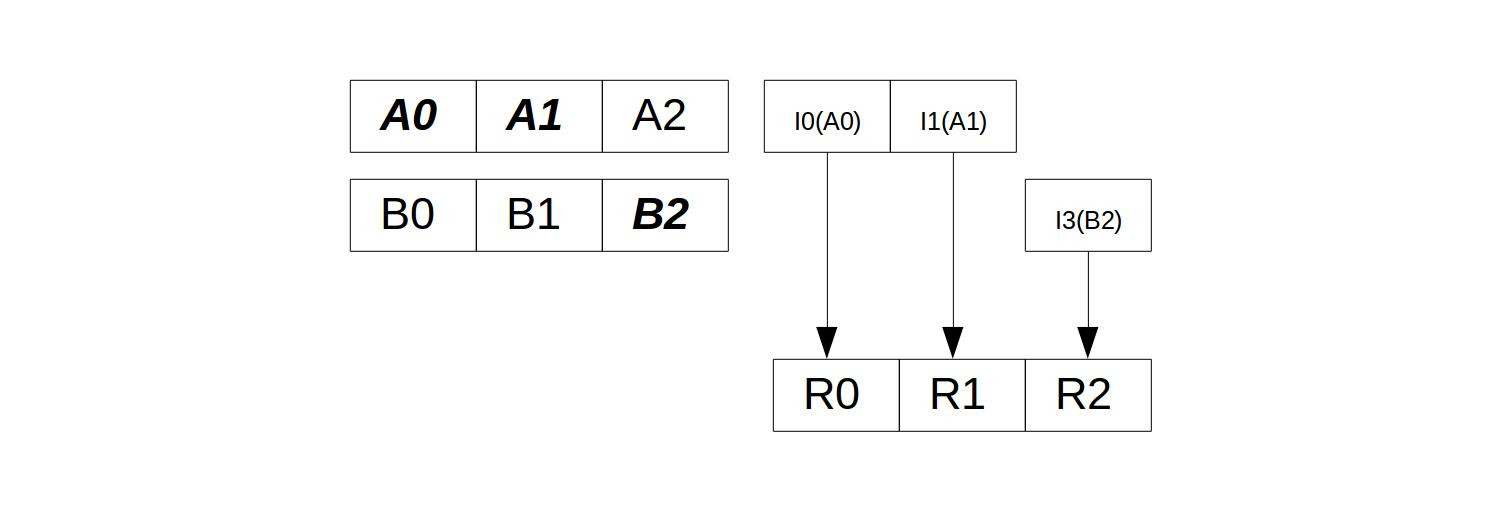
\includegraphics{img/update-transformation.jpg}
\caption{Update Transformation\label{fig:updatetransform}}
\end{figure}

Solange die Einfüge-Funktion \(Ix(Ex)\) eine Numerische Operation (+
oder -) ist, spielt es meist! Rolle in welcher Kausalität die Funktionen
auf dem Server angewendet werden.

\paragraph{Kontextbezogene Daten}\label{kontextbezogene-daten}

Kontextbezogene Daten können nur aktualisiert werden, wenn der Kontext
sich nicht geändert hat.

\paragraph{Unabhängige Daten}\label{unabhuxe4ngige-daten}

Unabhängige Daten können ohne Abhängigkeit des Zustandes anderer Daten
aktualisiert werden.\\Zu beachten ist, dass nur numerische, boolsche und
binäre Werte und nur die beiden Grundoperationen + und - immer
funktionieren.

\paragraph{Exklusive Daten}\label{exklusive-daten}

Für den Fall dass von 2 Geräten ein Update ausgeführt wird, müssen beide
Versionen gespeichert werden, und der User muss entscheiden welche
Version verwendet werden soll

\paragraph{Gemeinsame Daten}\label{gemeinsame-daten}

Im Falle von Text-Daten kann diese Art der Synchronisation nur für den
tatsächlichen Add verwendet werden.

\subsubsection{Wiederholbare
Transaktion}\label{wiederholbare-transaktion}

Statt nur einer Überführung einer Einzelnen Mutation in ein Insert wird
die gesamte Transaktion so gemacht.\\Falls nun eine Leseaktion auf eine
bereits mutiertes Objekt geschieht, welches noch nicht synchronisiert
wurde, und aufgrund dieser Lesekation eine andere Mutation passiert,
darf die zweite Mutation nur synchronisiert werden, falls die erste
Mutation auch erfolgreich war.

Es werden applikatorische Inkonsistenzen vermieden. Zusätzlich müssen
auf dem Client alle Lese- und Schreib-Operationen \enquote{ge-trackt}
werden.

\paragraph{Kontextbezogene Daten}\label{kontextbezogene-daten-1}

können in einer Transaktion, nur aktualisiert werden, wenn der Kontext
sich nicht geändert hat.

\paragraph{Unabhängige Daten}\label{unabhuxe4ngige-daten-1}

können ohne Abhängigkeit des Zustandes anderer Daten aktualisiert
werden.\\Zu beachten ist, dass nur numerische, boolsche und binäre Werte
und nur die beiden Grundoperationen + und - immer funktionieren.

\paragraph{Exklusive Daten}\label{exklusive-daten-1}

Für den Fall dass von 2 Geräten ein Update ausgeführt wird, müssen beide
Versionen gespeichert werden, und der User muss entscheiden welche
Version verwendet werden soll

\paragraph{Gemeinsame Daten}\label{gemeinsame-daten-1}

Im Falle von Text-Daten kann diese Art der Synchronisation nur für den
tatsächlichen Add verwendet werden.

\subsection{Konfliktauflösung}\label{konfliktaufluxf6sung}

Das Konzept der Konfliktauflösung beschäftigt sich mit der Auflösung von
Konflikten, die im Rahmen der Synchronisation aufgetreten sind.\\Da die
Beschaffenheit und Struktur der Daten, bei dieser Problemstellung eine
entscheidende Rolle einnehmen, ist im folgendn für jede
Klassifikations-Gruppe ein geeigneter Konfliktauflösungs-Algorithmus
aufgeführt.

\subsubsection{Zusammenführung (Merge)}\label{zusammenfuxfchrung-merge}

Einzelne Attribute oder Attributsgruppen innerhalb eines Objekts werden
als eigenständige Objekte betrachtet. So kann ein Konflikt, der auftritt
wenn zwei Objekte mit Mutationen in unterschiedlichen Attributsgruppen
synchronisiert werden , aufgelöst werden, indem nur die jeweils
mutierten Attributgrupen als synchronisationswürdig betrachtet werden.

Kontextbezogene Attribute sind in der selben Attributgruppe wie der
Kontext.

\begin{figure}[htbp]
\centering
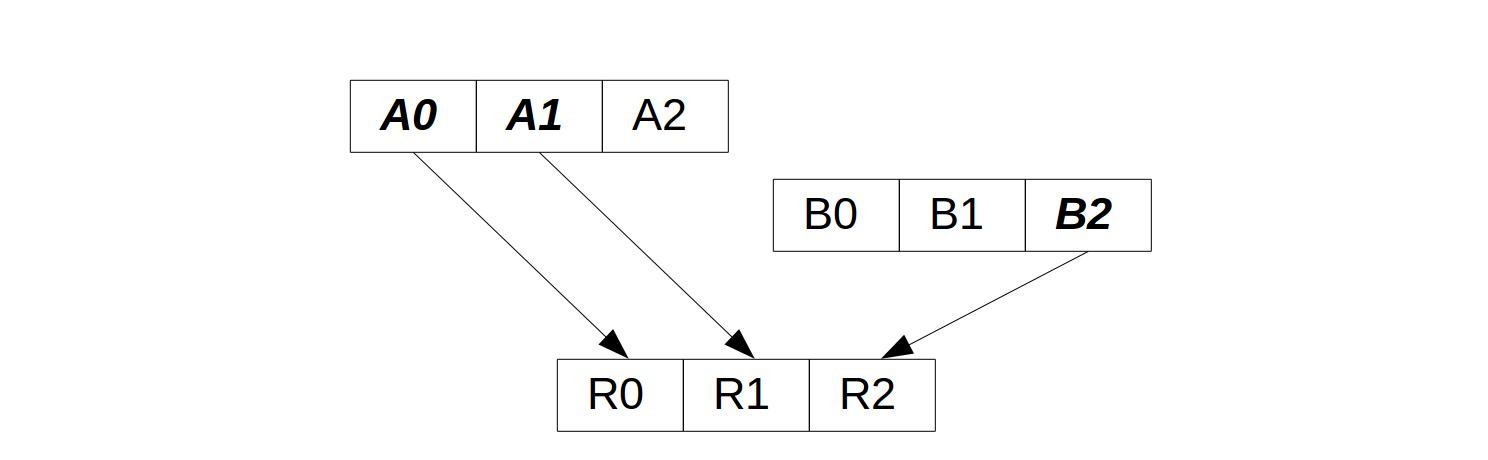
\includegraphics{./img/merge.jpg}
\caption{Merge}
\end{figure}

Diese Operation ist unabhängig von Datentyp, Struktur und Art.\\Der
(automatisierte) Merge kann nur durchgeführt werden, wenn nur eine
einzige Version eines Attributs existiert. -\textgreater{} nie
konkurrierende Versionen entstehen.

Darüber hinaus versieht der Server jede Attribut-Version mit einer
Versions-Nummer. So kann verhindert werden, dass ein Attribut mit einer
niederen Versions-Nummer über ein neueres Attribut synchronisiert wird.

\subsubsection{normalisierte Zusammenführung (Normalized
Merge)}\label{normalisierte-zusammenfuxfchrung-normalized-merge}

Wenn bei einer Synchronisierung mit zwei Objekten die selben Attribute
mutiert wurden, kann im Falle von numerischen Attributen, das Objekt mit
den geringsten Abweichungen vom Meridian über alle verfügbaren
Datensätze verwendet werden. Es wird also das normalisierteste Attribut
verwendet.\\Bei Attributsgruppen wird die Gruppe mit der insgesamt
geringsten Abweichung verwendet.\\Es muss eine Abstandsfunktion für
jedes Attribut oder jede Attributgruppe erstellt werden.

Es kann so die warscheinlichste Version verwendet werden. Wenn zu
\(t_1\) \(A_1\) und zu \(t_2\) \(A_2\), also das selbe Attribut
synchronisiert wird, wird es beide male angenommen. Beide Versionen
basieren auf der gleichen Ursprungsversion. \(A_2\) besitzt aber die
kleinere Abweichung und gewinnt deshalb.\\Hätte es die grössere
Abweichung, würde es nicht synchronisiert werden.

\section{Multistate}\label{multistate}

Der Zustand des Systems wird durch eine Message-Queue repräsentiert.

\begin{enumerate}
\def\labelenumi{\arabic{enumi}.}
\itemsep1pt\parskip0pt\parsep0pt
\item
  Message gets sent
\item
  Message gets enqueued
\item
  If message conflicts with an other message -\textgreater{} next else
  -\textgreater{} end
\item
  message gets moved bevore conflicts
\item
  Fork is generated
\item
  It is decided with fork is the main fork (master)
\end{enumerate}

Zu jedem Zeitpunkt sind beliebig viele gültige Stati erlaubt.\\Es gibt
zu jedem echten Zeitpunkt nur einen einzigen gültigen Status (main
fork), bei Konflikten kann aber ein anderer Zweig nachträglich als
Master definiert werden.

Jedem Benutzer/Session werden gegebenenfalls eigene Zweige zugewiesen.
Das integrieren der Zweite in den Master-Zweig muss manuell vorgenommen
werden.

Weiter werden alle neu eingehende Nachrichten für alle Zweige
verarbeitet, ausser es entstünden dadurch weitere Konflikte.

Es können also immer alle Änderungen synchronisiert werden. Keine
Mutationen gehen verloren.\\Die Konfliktauflösung kann nachträglich
durchgeführt werden.

Wenn Nachrichten eingespielt werden, die Konflikte auflösen, kann ein
anderer Zweig als Master markiert werden, dadurch können nachträglich
andere Konflikte ausgelöst werden etc.

Z.B. das Resultat der Abfrage des Status gestern um 10:00 muss nicht dem
Resultat der Abfrage von heute, wie der Status gestern um 10:00 war.

Jeder Status ist also Rückwirkend veränderbar. Entsprechende Systeme
müssen dafür ausgelegt sein.

Die Konfliktauflösung funktioniert genau gleich wie bei den Singlestate
Systemen. Wir dürfen jedoch sehr fiel mehr \enquote{greedy} sein.

Statt das wahrscheinlichsten oder des erste eingehenden Attribut zu
verwenden wird die Kausalität sichergestellt. So wird für jede Mutation
ein \enquote{quasi} Timestamp generiert (auch auf den mobilen
Endgeräten) um so den Zeitpunkt der Synchronisierung zu egalisieren.
Mutationen die echt zu erst durchgeführt wurden, gelten.

\begin{figure}[htbp]
\centering
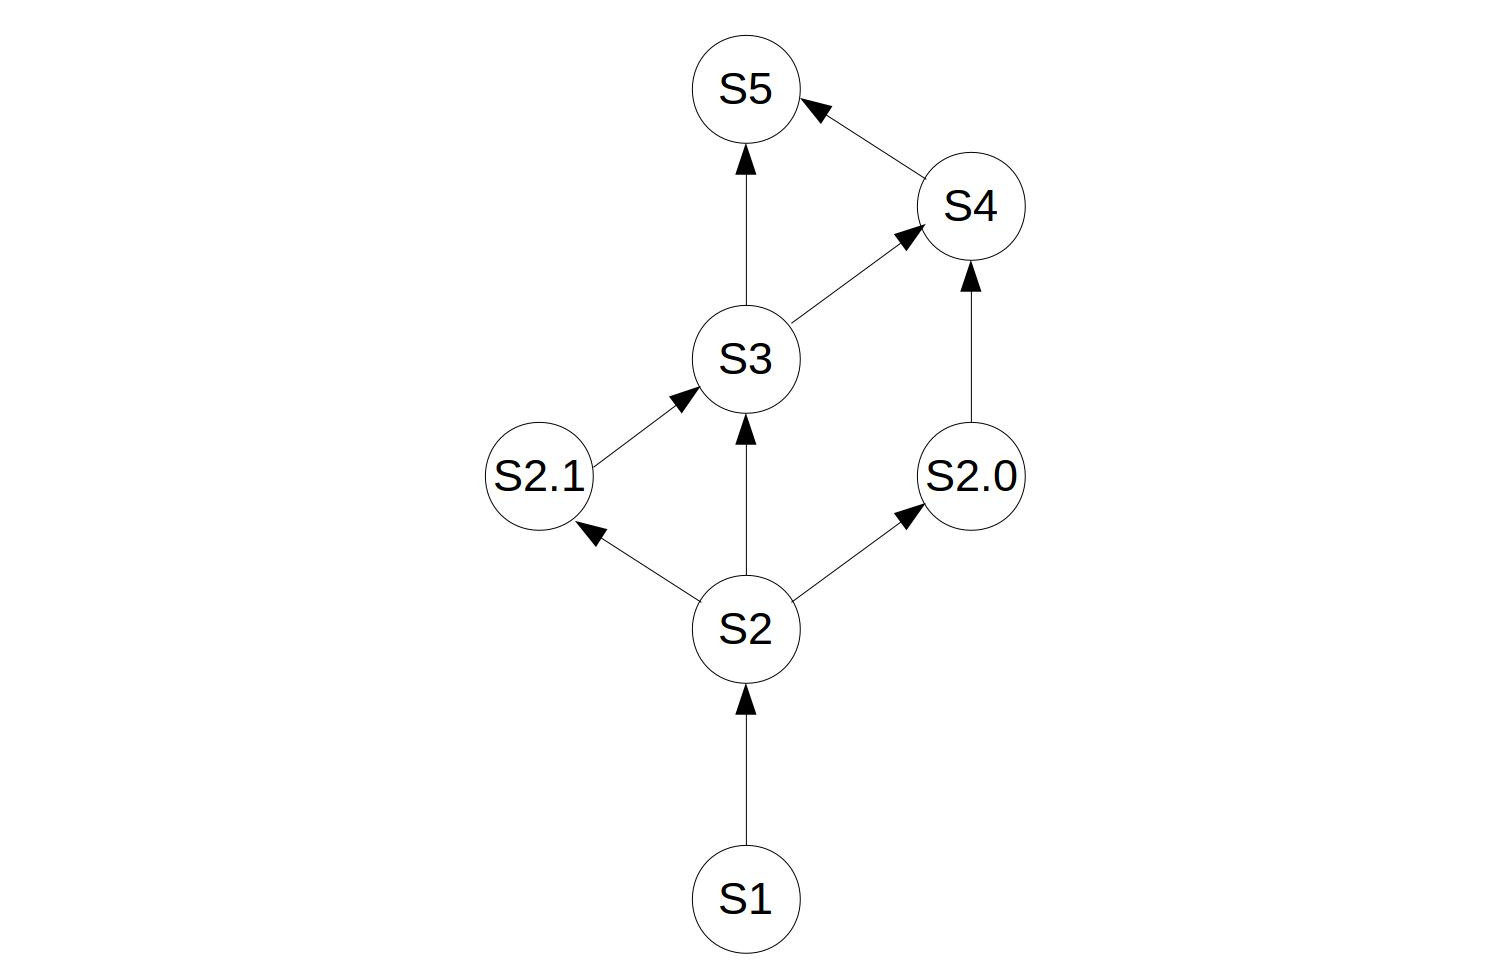
\includegraphics{img/states_01.jpg}
\caption{Multistate}
\end{figure}

\subsection{Gesamtkonzept}\label{gesamtkonzept}

Das Gesamtkonzept besteht in einer Zusammenführung aller bereits
erwähnter Konzepte. Je nach zu synchronisierendem Datenbestand müssend
entsprechend Passende Lösungsverfahren angewendet werden.

\chapter{Design des Prototypen}\label{design-des-prototypen}

In diesem Kapitel werden die aus dem Kapitel \hyperref[konzept]{Konzept}
gewonnenen Erkenntnisse umgesetzt.

\section{Design-Ansätze}\label{design-ansuxe4tze}

Zur Lösung der Aufgabenstellung wurden drei Design-Ansätze erarbeitet.
Diese werden folgend kurz erläutert.

\subsection{Server zentrierte
Architektur}\label{server-zentrierte-architektur}

Der Server führt alle Berechnungen o.ä. durch. Nur mit einer aktiven
Verbindung zum Server können Manipulationen am Datenbestand durchgeführt
werden.

\subsection{Client zentrierte
Architektur}\label{client-zentrierte-architektur}

Der Client trifft Entscheidungen und führt die Berechtigungsprüfung
durch. Die Resultate werden dann dem Server übermittelt.

\subsection{Client zentrierte, Server basierte
Architektur}\label{client-zentrierte-server-basierte-architektur}

Der Client simuliert alle Manipulationen. Der Server entscheidet über
das Resultat.

\section{Entscheid}\label{entscheid}

Anforderung UC 5-8 =\textgreater{} \{Client zentrierte, Server basierte
Architektur, Message Oriented\}

\section{Design}\label{design}

Der Prototyp besteht aus 3 Bausteinen; Server, API und Client.

\begin{figure}[htbp]
\centering
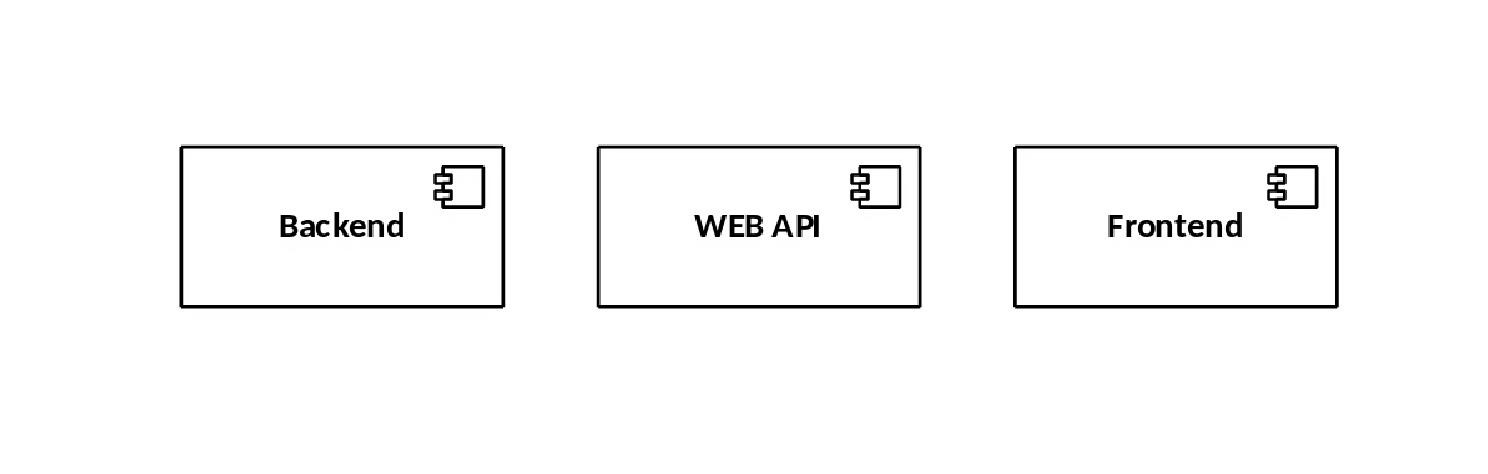
\includegraphics{img/design_components.jpg}
\caption{Bausteinübersicht\label{fig:bausteinübersicht}}
\end{figure}

Die Bausteine werden in den folgenden Kapitel erläutert.

\subsection{Backend}\label{backend}

Alle Daten müssen zur Aufbereitung in das Backend transferiert
werden.\\Im Backend wird zwischen Persistenz- und Logik-Schicht
unterschieden.

\subsubsection{Logik}\label{logik}

Die Logik-Schicht nimmt alle Nachrichten entgegen und führt, sofern
aufgetreten Konfliktauflösungen vor.\\Die Kommunikation mit der API
findet nur über Nachrichten statt.\\Die Kommunikation mit der darunter
liegenden Persistenz-Schicht findet über eine Asynchrone API statt.

S\_LOGIC\_SM\_get\\S\_LOGIC\_SM\_create\\S\_LOGIC\_SM\_update\\S\_LOGIC\_SM\_delete

\subsubsection{Persistenz}\label{persistenz}

Die Persistenz soll Modell-Basiert sein.

\subsection{API}\label{api}

Message Queuing \& Message Passing - nothing else

Umsetzung mit REST-Like Verhalten (get,put,update,delete)

\textbf{Client-Side}\\S\_API\_WEB\_get\\S\_API\_WEB\_put\\S\_API\_WEB\_update\\S\_API\_WEB\_delete

\textbf{Server-Side}\\S\_API\_WEB\_send

\subsection{Frontend}\label{frontend}

Der Client bietet keine Persistenz über einen Neustart hinweg.

\begin{figure}[htbp]
\centering
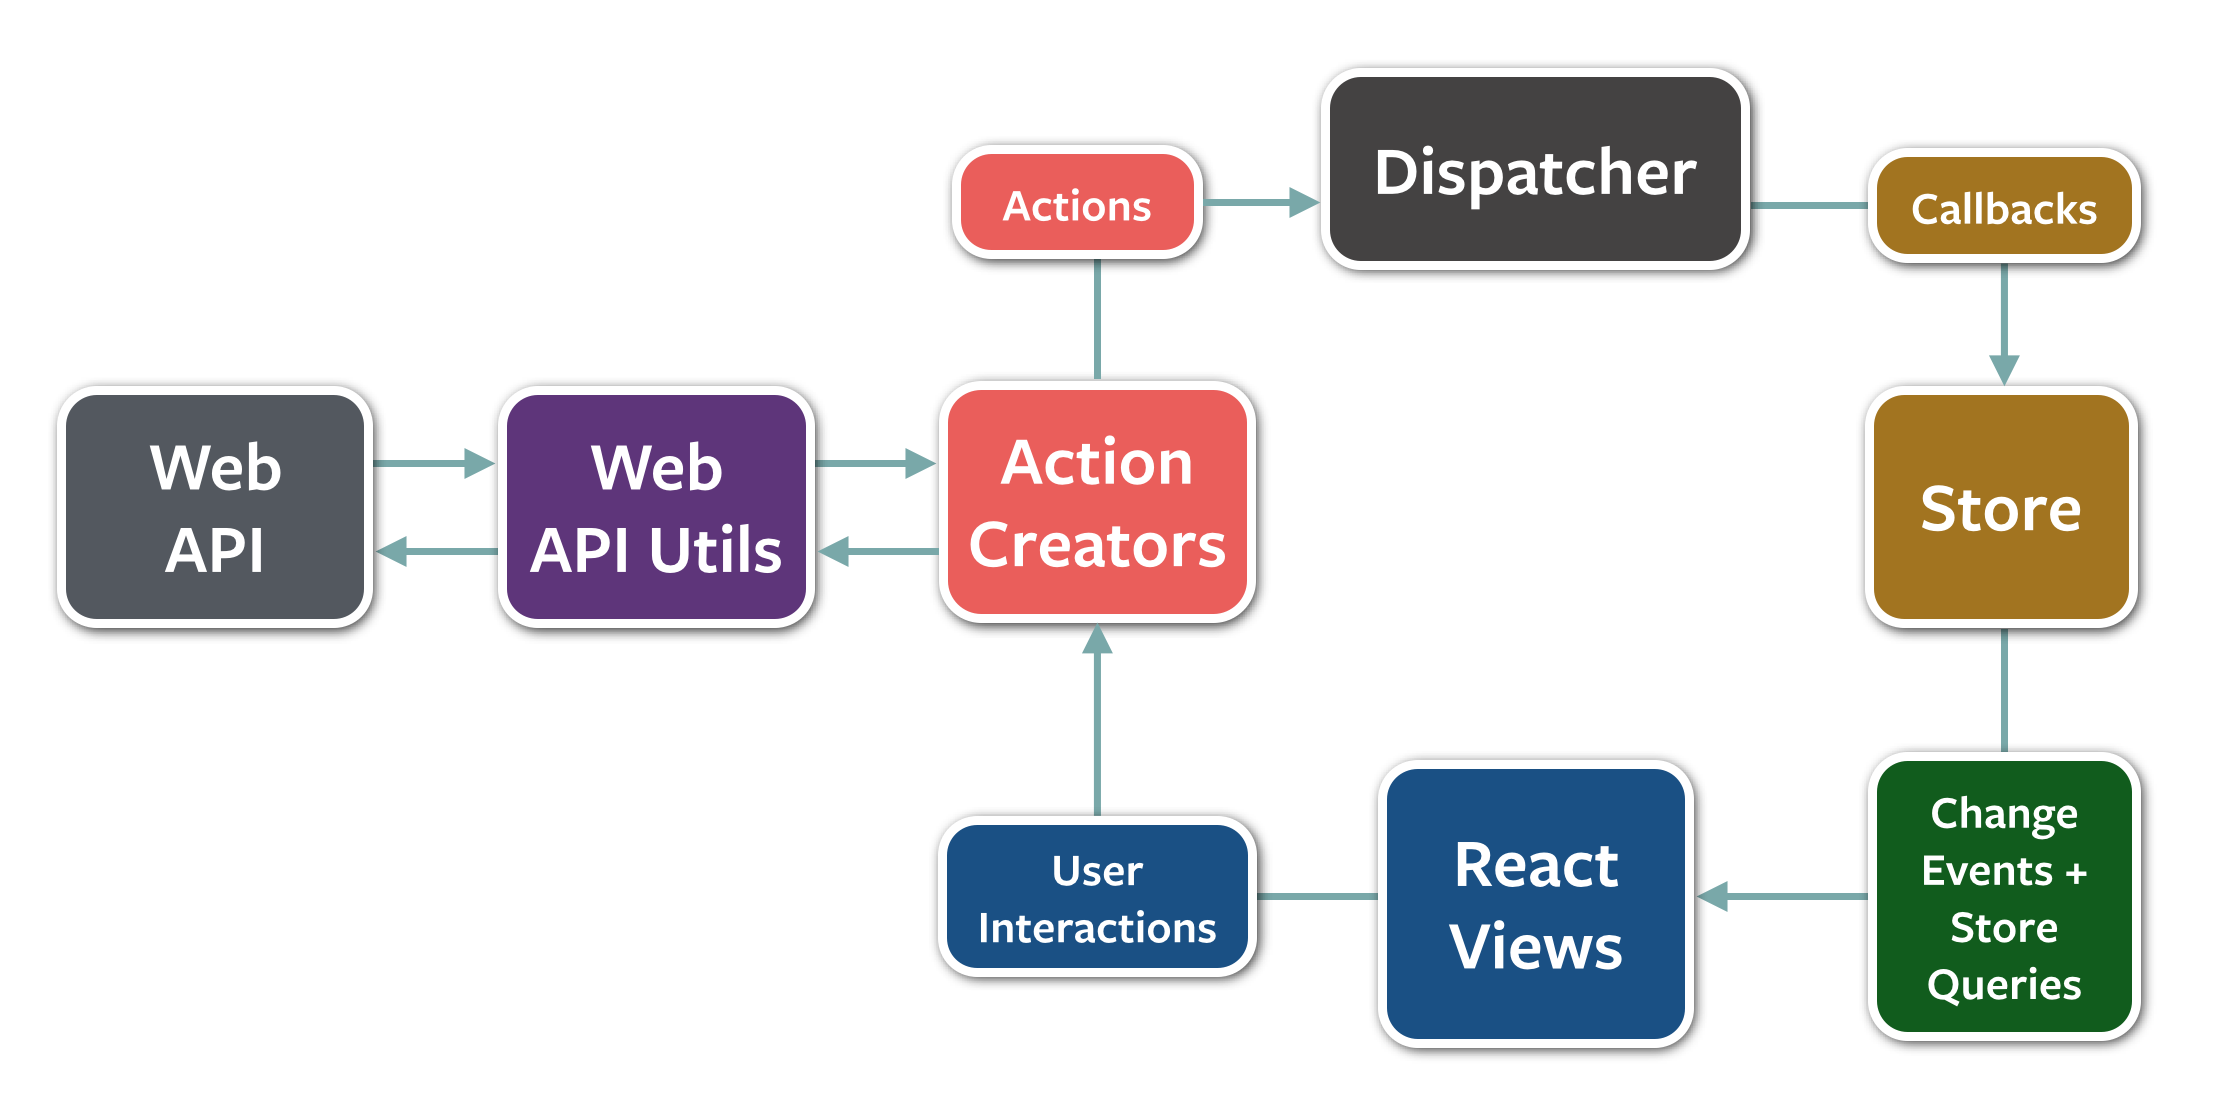
\includegraphics{img/flux-diagram.png}
\caption{Flux Diagramm}
\end{figure}

C\_PRES\_STORE\_update\\C\_PRES\_STORE\_delete

\subsection{Message Flow}\label{message-flow}

Frontend \textless{}-\textgreater{} API \textless{}-\textgreater{}
Backend

Frontend: ActionCreator -\textgreater{} Dispatcher -\textgreater{} Store
-\textgreater{} API -\textgreater{} ActionCreator

API: Queue -\textgreater{} Transporter

Backend: API -\textgreater{} Logiclayer -\textgreater{} API

\subsection{AMD Pattern}\label{amd-pattern}

Asyncronous module definition (AMD) ist eine JavaScript API um Module zu
definieren und diese zur Laufzeit zu laden. Dadurch können
Javascript-lastige Webseiten beschleunigt werden, da Module erst geladen
werden, wenn sie gebraucht werden. Weiter werden durch den Loader die
Module gleichzeitig geladen, dadurch kann die Bandbreite voll ausgenutzt
werden.\\Da die Module durch die Vorgabe des Patterns in einzelnen
Dateien abgelegt sind, wird eine Kapselung ähnlich wie bei Java
erreicht. Das erleichtert die Fehlersuche und erhöht die
Verständlichkeit des Programmes drastisch. Auch die Wiederverwendbarkeit
der Module wird dadurch erhöht.\\Da in jedem Modul die Abhängigkeiten
definiert werden müssen, kann während dem Build-Prozess die
Abhängigkeiten geprüft werden, um so die Verfügbarkeit aller benötigten
Module sicher zu stellen.

\section{Beispielapplikation}\label{beispielapplikation}

Gem. Aufgabenstellung soll der Prototyp anhand eines passenden
Fallbeispiel die Funktionsfähigkeit Zeigen.

Die Beispielapplikation soll eine Ressourcenplan-Software sein.
Folgendes soll möglich sein:

\begin{enumerate}
\def\labelenumi{\arabic{enumi}.}
\itemsep1pt\parskip0pt\parsep0pt
\item
  einen neuen Raum erfassen (Name, Grösse, Anzahl Sitze)
\item
  einen bestehenden Raum anpassen/löschen
\item
  einen Termin auf einem Raum Buchen (Name, Zeit\&Datum,
  Kurzbeschreibung, Besucherliste, persönliche Notizen)
\item
  einen Bestehenden Termin anpassen/absagen
\end{enumerate}

\chapter{Prototyp}\label{prototyp}

Dieses Kapitel adressiert die Implementation des Prototypen gemäss den
Anroderungen aus Kapitel \hyperref[analyse]{Analyse}.

\section{Umsetzung}\label{umsetzung}

\section{Technologie Stack}\label{technologie-stack}

\begin{longtable}[c]{@{}ll@{}}
\toprule
\begin{minipage}[b]{0.26\columnwidth}\raggedright\strut
Software
\strut\end{minipage} &
\begin{minipage}[b]{0.63\columnwidth}\raggedright\strut
Beschreibung/Auswahlgrund
\strut\end{minipage}\tabularnewline
\midrule
\endhead
\begin{minipage}[t]{0.26\columnwidth}\raggedright\strut
\textbf{Grunt}
\strut\end{minipage} &
\begin{minipage}[t]{0.63\columnwidth}\raggedright\strut
Grunt ermöglicht es dem Benutzer vordefinierte Tasks von der
Kommandozeile aus durchzuführen. So sind Build- und Test-Prozesse für
alle Benutzer ohne detaillierte Kenntnisse durchführbar.\\Da Grunt eine
sehr grosse Community besitzt und viele Plugins sowie hervorragende
Dokumentationen verfügbar, wurde Grunt eingesetzt.
\strut\end{minipage}\tabularnewline
\begin{minipage}[t]{0.26\columnwidth}\raggedright\strut
\textbf{Karma}
\strut\end{minipage} &
\begin{minipage}[t]{0.63\columnwidth}\raggedright\strut
\strut\end{minipage}\tabularnewline
\begin{minipage}[t]{0.26\columnwidth}\raggedright\strut
\textbf{CoffeeScript}
\strut\end{minipage} &
\begin{minipage}[t]{0.63\columnwidth}\raggedright\strut
\strut\end{minipage}\tabularnewline
\begin{minipage}[t]{0.26\columnwidth}\raggedright\strut
\textbf{RequireJS}
\strut\end{minipage} &
\begin{minipage}[t]{0.63\columnwidth}\raggedright\strut
RequireJS ermöglicht die Implementierung des AMD Pattern.Dadurch können
auch in JavaScript Code-Abhängigkeiten definiert werden. Zusammen mit
r.js kann dies bereits zur Compilierzeit geprüft werden.\\Da weder
Backbone noch Django über eine Depencency-Control für JavaScript
verfügen, setze ich RequireJS ein.
\strut\end{minipage}\tabularnewline
\begin{minipage}[t]{0.26\columnwidth}\raggedright\strut
\textbf{ReactJS}
\strut\end{minipage} &
\begin{minipage}[t]{0.63\columnwidth}\raggedright\strut
\strut\end{minipage}\tabularnewline
\begin{minipage}[t]{0.26\columnwidth}\raggedright\strut
\textbf{FluxifyJS}
\strut\end{minipage} &
\begin{minipage}[t]{0.63\columnwidth}\raggedright\strut
\strut\end{minipage}\tabularnewline
\begin{minipage}[t]{0.26\columnwidth}\raggedright\strut
\textbf{SequelizeJS}
\strut\end{minipage} &
\begin{minipage}[t]{0.63\columnwidth}\raggedright\strut
\strut\end{minipage}\tabularnewline
\begin{minipage}[t]{0.26\columnwidth}\raggedright\strut
\textbf{Express}
\strut\end{minipage} &
\begin{minipage}[t]{0.63\columnwidth}\raggedright\strut
\strut\end{minipage}\tabularnewline
\begin{minipage}[t]{0.26\columnwidth}\raggedright\strut
\textbf{Socket.io}
\strut\end{minipage} &
\begin{minipage}[t]{0.63\columnwidth}\raggedright\strut
\strut\end{minipage}\tabularnewline
\bottomrule
\end{longtable}

\section{Entwicklungsumgebung}\label{entwicklungsumgebung}

Grunt + Karma = All you need

\section{Entwicklung}\label{entwicklung}

Verwendung vom Socket io (Namespaces etc)\\Tricks mit API \& Message
Routing, binding to io.on \enquote{message} -\textgreater{}
flux.doAction

Express Server:\\Statisches Daten -\textgreater{} Frontend /\\Socket.io
-\textgreater{} /socket.io\\Message-Bus -\textgreater{} Fluxify also in
the backend

RequireJS Modules testable in the Browser :-D

Stores in the Frontend\\Models in the Backend

\section{Grafische Umsetzung
Fallbeispiel}\label{grafische-umsetzung-fallbeispiel}

\chapter{Testing}\label{testing}

\section{Unit-Testing}\label{unit-testing}

\section{Integration-Testing}\label{integration-testing}

\section{Test der Akzeptanzkriterien}\label{test-der-akzeptanzkriterien}

\section{Überprüfung der
Aufgabenstellung}\label{uxfcberpruxfcfung-der-aufgabenstellung}

\part[Teil iv]{Abschluss und Ausblick}

\chapter{Review}\label{review}

\section{Testing}\label{testing-1}

\subsection{Integrationstest}\label{integrationstest}

\subsection{Systemtest}\label{systemtest}

\section{Validation}\label{validation}

\subsection{Test der
Akzeptanzkriterien}\label{test-der-akzeptanzkriterien-1}

\subsection{Überprüfung der
Aufgabenstellung}\label{uxfcberpruxfcfung-der-aufgabenstellung-1}

\chapter{Ausblick}\label{ausblick}

\chapter{Fazit und Schlusswort}\label{fazit-und-schlusswort}

\appendix

\chapter{Appendix}\label{appendixA}

\hyperdef{}{glossar}{\section{Glossar}\label{glossar}}

\hyperdef{}{appendixux5faufgabenstellung}{\section{Aufgabenstellung}\label{appendixux5faufgabenstellung}}

\subsection{Thema}\label{thema}

Zeil der Arbeit ist es verschiedene Konfliktlösungsverfahren bei
Multi-Master Datenbanksystemen zu untersuchen.

\subsection{Ausgangslage}\label{ausgangslage}

Mobile Applikationen (Ressourcen-Planung, Ausleihlisten, etc.) gleichen
lokale Daten mit dem Server ab. Manchmal werden von mehreren
Applikationen, gleichzeitig, dieselben Datensätze mutiert. Dies kann zu
Konflikten führen. Welche Techniken und Lösungswege können angewendet
werden, damit Konflikte gelöst werden können oder gar nicht erst
auftreten?

\subsection{Ziele der Arbeit}\label{ziele-der-arbeit}

Das Ziel der Bachelorthesis besteht in der in der Konzeption und der
Entwicklung eines lauffähigen Software-Prototypen, welcher mögliche
Synchronisations- und Konfliktlösungsverfahren von Clientseitiger und
Serverseitiger Datenbank demonstriert. Im Speziellen, soll gezeigt
werden, welche Möglichkeiten der Synchronisation beim Einsatz von
mobilen Datenbanken (Web-Anwendungen) bestehen, so dass die
Clientseitige Datenbank auch ohne Verbindung zum Server mutiert und erst
zu einem späteren Zeitpunkt synchronisiert werden kann, ohne dass
Inkonsistenzen auftreten. Die Art und Funktionsweise des
Software-Prototyp soll in einer geeigneten Form gewählt werden, so dass
verschiedene Synchronisations- und Konfliktlösungsverfahren an ihm
gezeigt werden können. Der Software-Prototyp soll nach denen, im
Unterricht behandelten Vorgehensweisen des Test Driven Development (TDD)
entwickelt werden.

\subsection{Aufgabenstellung}\label{aufgabenstellung-1}

\textbf{A1 Recherche:}

\begin{itemize}
\itemsep1pt\parskip0pt\parsep0pt
\item
  Definition der Fachbegriffe
\item
  Erarbeitung der technischen Grundlagen zur Synchronisation von
  Datenbanken und Datenspeichern
\end{itemize}

\textbf{A2 Analyse:}

\begin{itemize}
\itemsep1pt\parskip0pt\parsep0pt
\item
  Analyse der Synchronisationsverfahren und deren Umgang mit Konflikten
\item
  Analyse der Synchronisationsverfahren im Bereich der Web-Anwendungen
\item
  Durchführen einer Anforderungsanalyse an die Software
\end{itemize}

\textbf{A3 Konzept:}

\begin{itemize}
\itemsep1pt\parskip0pt\parsep0pt
\item
  Erstellen eines Konzepts der Software
\item
  Erstellen eines Konzepts der Implementierung zweier ausgewählten
  Synchronisations-Verfahren
\end{itemize}

\textbf{A4 Prototyp:}

\begin{itemize}
\itemsep1pt\parskip0pt\parsep0pt
\item
  Konzeption des Prototypen der die gestellten Anforderungen erfüllt
\item
  Entwickeln des Software-Prototyps
\item
  Implementation zweier ausgewählter Synchronisations- und
  Konfliktlösungsverfahren
\end{itemize}

\textbf{A5 Review:}

\begin{itemize}
\itemsep1pt\parskip0pt\parsep0pt
\item
  Test des Prototyps und Protokollierung der Ergebnisse
\end{itemize}

\subsection{Erwartete Resultate}\label{erwartete-resultate}

\textbf{R1 Recherche:}

\begin{itemize}
\itemsep1pt\parskip0pt\parsep0pt
\item
  Glossar mit Fachbegriffen
\item
  Erläuterung der bereits bekannten Synchronisation- und
  Konfliktlösungs-Verfahren, sowie deren mögliches Einsatzgebiet
\end{itemize}

\textbf{R2 Analyse:}

\begin{itemize}
\itemsep1pt\parskip0pt\parsep0pt
\item
  Dokumentation der Verfahren und deren Umgang mit
  Synchronisation-Konflikten (Betrachtet werden nur MySQL, MongoDB)
\item
  Dokumentation der Verfahren zur Synchronisation im Bereich von
  Web-Anwendungen (Betrachtet werden nur die Frameworks Backbone.js und
  Meteor.js)
\item
  Anforderungsanalyse der Software
\end{itemize}

\textbf{R3 Konzept:}

\begin{itemize}
\itemsep1pt\parskip0pt\parsep0pt
\item
  Dokumentation des Konzepts der Software
\item
  Dokumentation der Umsetzung der ausgewählten
  Synchronisations-Verfahren
\end{itemize}

\textbf{R4 Prototyp:}

\begin{itemize}
\itemsep1pt\parskip0pt\parsep0pt
\item
  Dokumentation des Prototypen
\item
  Implementation des Prototypen gemäss Konzept und Anforderungsanalyse
\item
  Implementation zweier ausgewählter Synchronisations- und
  Konfliktlösungsverfahren
\end{itemize}

\textbf{R5 Review:}

\begin{itemize}
\itemsep1pt\parskip0pt\parsep0pt
\item
  Protokoll der Tests des Software Prototypen
\end{itemize}

\chapter{Verzeichnisse}\label{verzeichnisse}

\section{Quellenverzeichnis}\label{quellenverzeichnis}

\vspace*{-2.5cm}\renewcommand{\bibname}{}\begingroup \let\clearpage\relax
\printbibliography
\endgroup

\section{Tabellenverzeichnis}\label{tabellenverzeichnis}

\renewcommand{\listtablename}{} 

\begingroup \let\clearpage\relax
\listoftables
\endgroup

\section{Abbildungsverzeichnis}\label{abbildungsverzeichnis}

\renewcommand{\listfigurename}{} 

\begingroup\let\clearpage\relax
\listoffigures
\endgroup


\end{document}